\begin{frame}[fragile]{Uso de Canvas View en Android}
\textbf{¿Qué es un Canvas View?}

\begin{itemize}
    \item Permite dibujar gráficos personalizados directamente en pantalla.
    \item Se utiliza extendiendo la clase \texttt{View} y sobrescribiendo el método \texttt{onDraw()}.
    \item Ideal para juegos, visualizaciones y dibujo libre.
\end{itemize}


\textbf{Métodos principales:}
\begin{itemize}
    \item \textbf{onDraw(Canvas canvas):} Método donde se realiza el dibujo.
    \item \textbf{invalidate():} Solicita redibujar la vista.
    \item \textbf{onTouchEvent():} Maneja interacción táctil.
\end{itemize}


\textbf{Clases importantes:}
\begin{itemize}
    \item \textbf{Canvas:} Superficie de dibujo.
    \item \textbf{Paint:} Define color, estilo y grosor.
    \item \textbf{Path:} Permite dibujar formas complejas.
\end{itemize}


\textbf{Ventajas:}
\begin{itemize}
    \item Alto control sobre gráficos.
    \item Ideal para interfaces personalizadas.
\end{itemize}

\end{frame}



\begin{frame}[fragile]
\frametitle{Demo 16: CanvasView }
\begin{columns}
\column{0.80\linewidth}

\scriptsize
Del Repositorio Github:
\begin{itemize}
%\item Agregar la siguiente linea: \textit{implementation("com.github.PhilJay:MPAndroidChart:v3.1.0")}, al final de la seccion Dependencies del archivo Build.graddle.kts (Module: App).
%\item Agregar la siguiente linea: \textit{maven \{ url = uri(``https://jitpack.io'') \}}, al final de la seccion \textit{dependencyResolutionManagement } del archivo settings.graddle.kts.
\item Copiar el archivo \textit{MainActivity\_Demo16.java} (dentro del Folder códigosJAVA) al mismo directorio donde esta el MainActivity.java
\item Copiar el archivo \textit{CanvasView.java} (dentro del Folder códigosJAVA) al mismo directorio donde esta el MainActivity.java

\item Copiar el archivo \textit{activity\_main\_demo16.xml} (dentro del Folder Carpeta\_layout) al mismo directorio donde esta el activity\_main.xml
\item Modificar dentro del archivo \textit{activity\_main\_demo16.xml} la cadena \textit{.com.example.a2026\_01\_holamundoandroid.CanvasView} por \textit{$<$SuPackage$>$.CanvasView}.
\item Modificar en el archivo \textit{AndroidManifest.xml} la cadena \textit{.MainActivity\_Demo15} por \textit{.MainActivity\_Demo16}.


%\item Ir a la linea 22 de archivo del archivo \textit{MainActivity\_Demo09.java}, poner el cursos en la palabra (en Rojo) \textit{documentfile}, presionar la combinación ALT+ENTER, y seleccionar de la lista desplegable la opcion ``Add dependency on ....''. Esto quitará el error y hara los ajustes necesarios. 
\end{itemize}

%\begin{block}{Demo \#09}
%Un App que permite escribir el contenido de un EditText a un archivo y cargar el contenido de cualquier archivo en el EditText
%\end{block}


\column{0.20\linewidth}

\begin{center}
 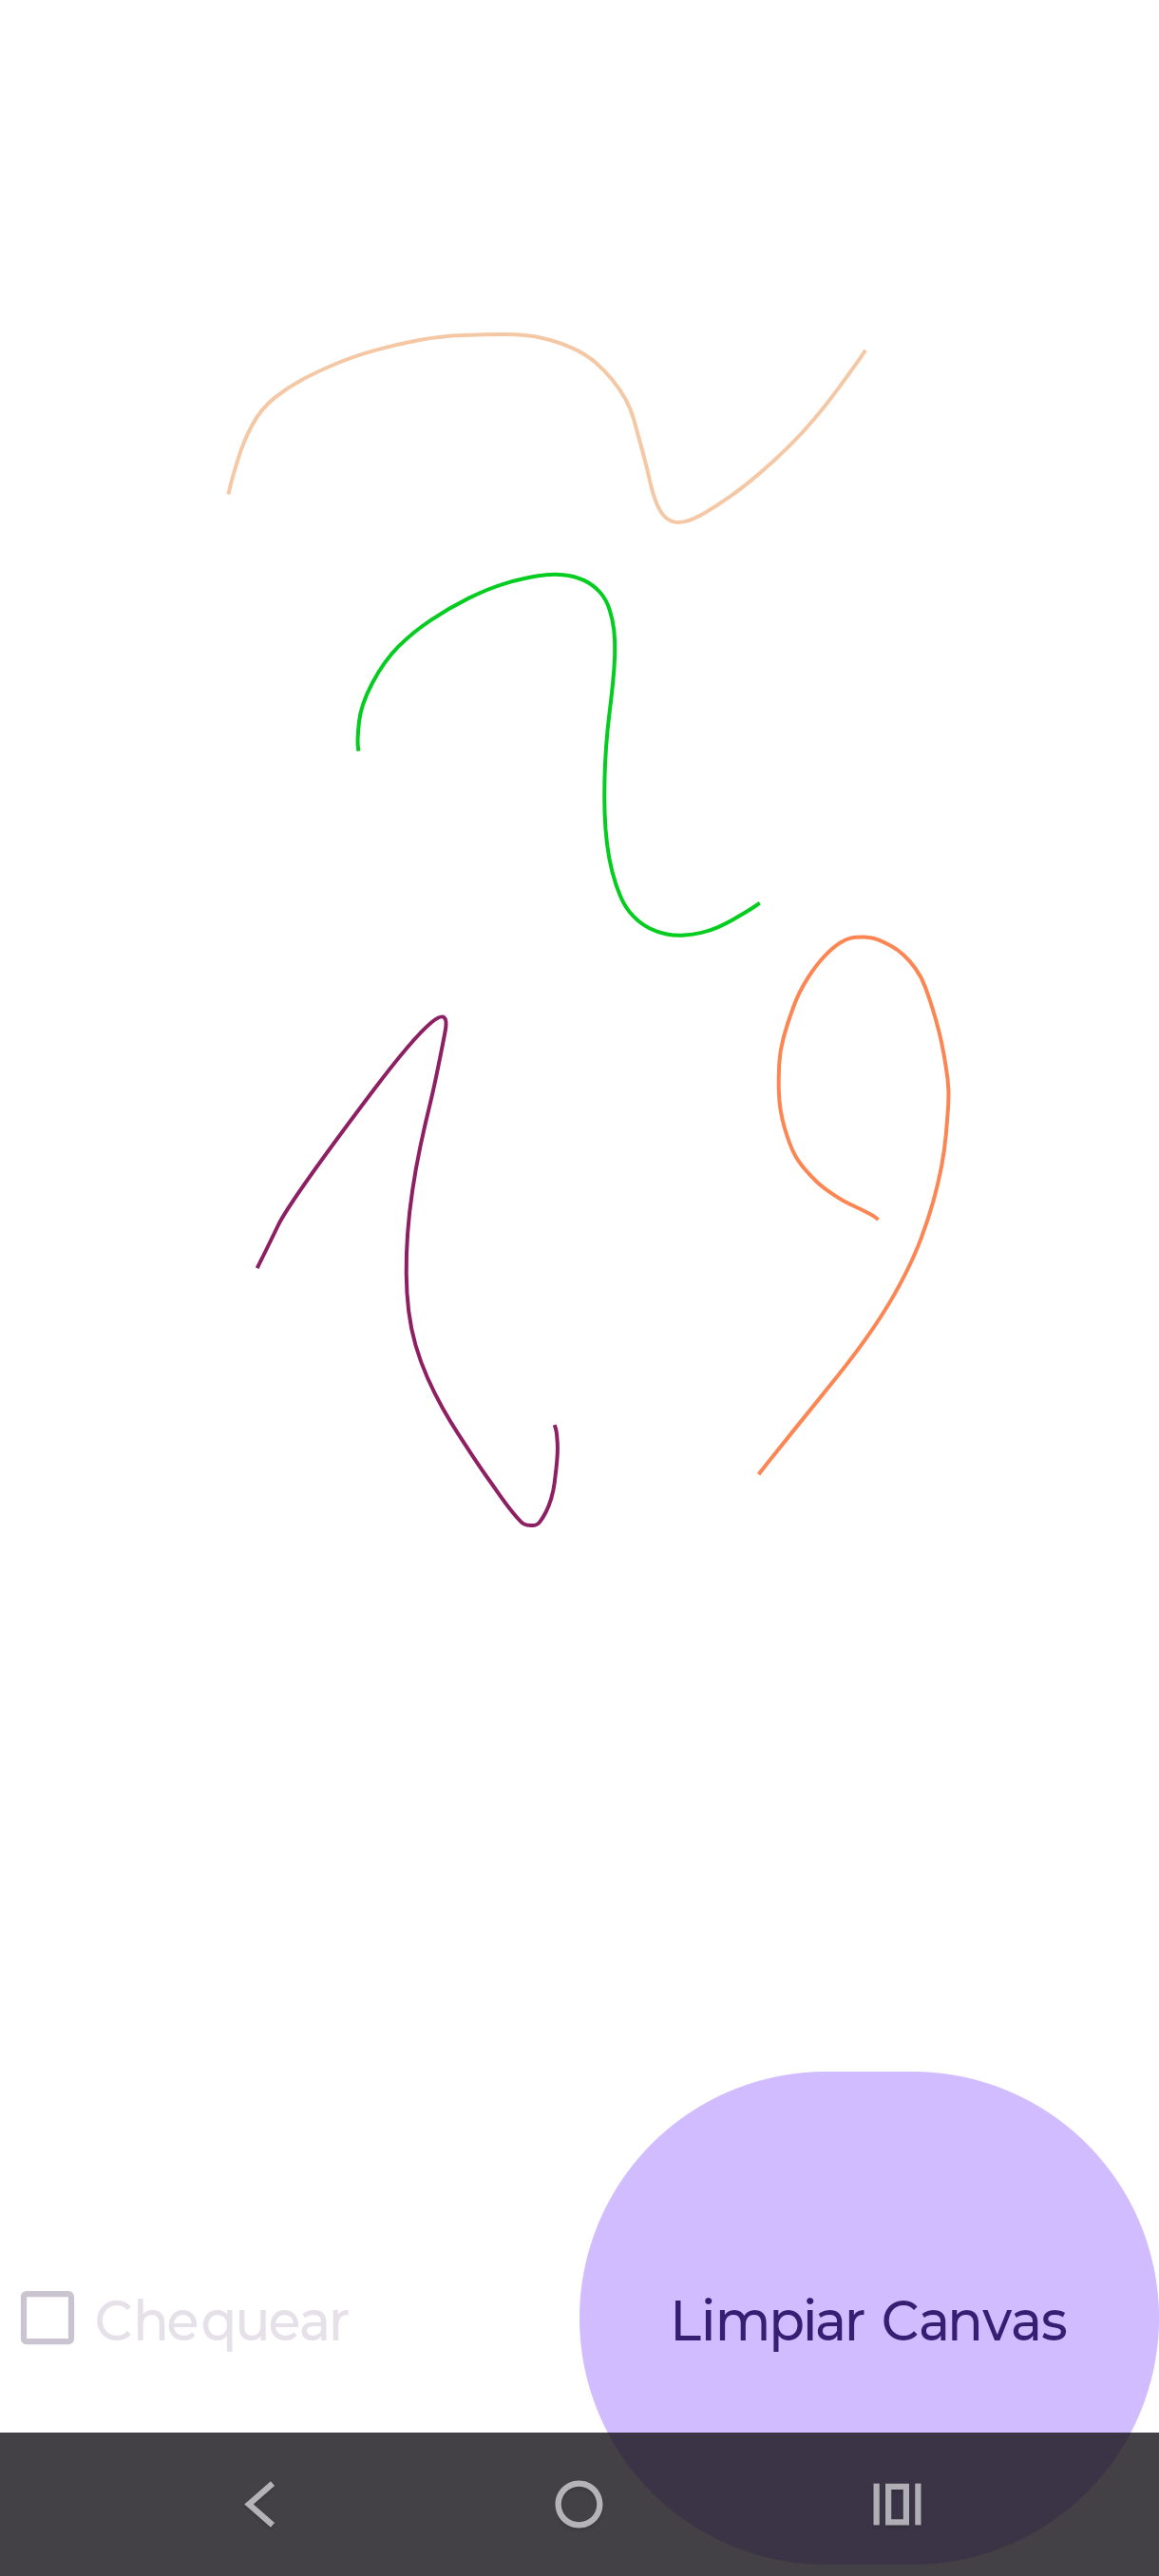
\includegraphics[width=0.98\textwidth]{02_TallerCBTis/figs/Demo16}
\end{center}

\end{columns}

\end{frame}

